\documentclass[]{article}
\usepackage[spanish.mexico]{babel}
\usepackage[T1]{fontenc}
\usepackage[utf8]{inputenc}
%\usepackageB.\\{lmodern}
\usepackage[a4paper]{geometry}

%\usepackage{natbib}
\usepackage{cite}


%Grafico de barras
\usepackage{pgfplots}

%Graficos e imagenes
\usepackage{graphicx}


%\title{Proyecto de Optimización de Energía}
%\author{Pablo Vivar Colina}
%\date{Mayo 2018}



\begin{document}
	
	%\usepackage[top=2cm,bottom=2cm,left=1cm,right=1cm]{geometry}


\begin{titlepage}
     \begin{center}
	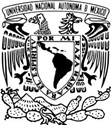
\includegraphics[width=0.09\textwidth]{UNAM}\Large Universidad Nacional Autónoma de México
        	
\includegraphics[width=0.09\textwidth]{FI}\\[1cm]
        \Large Facultad de Ingeniería\\[1cm]
       % \Large División de Ciencias Básicas\\[1cm]
         \Large Laboratorio de Fundamentos de Control(6655)\\[1cm]
         %la clave antes era:4314
         \footnotesize Profesor: Salcedo Ubilla María Leonor Ing.\\[1cm]
        \footnotesize Semestre 2019-1\\[1cm]
        
       

        \Large Práctica No. 1\\[1cm]
        
           

\Large Introdcción MATLAB
        
         %Texto a la derecha
          \begin{flushright}
\footnotesize  Grupo 2\\[0.5cm]
\footnotesize Brigada: 4\\[0.5cm]
\footnotesize Rodrigo Adrián Martínez López\\[0.5cm]
\footnotesize Vivar Colina Pablo\\[0.5cm]
 \end{flushright}
    %Texto a la izquierda
          \begin{flushleft}
        \footnotesize Ciudad Universitaria Agosto de 2018.\\
          \end{flushleft}
         
          
        %\vfill
        %\today
   \end{center}
\end{titlepage}
 %agregar portada

%\maketitle

%\tableofcontents  % Write out the Table of Contents

%\listoffigures  % Write out the List of Figures


\section{Introducción}

Prueba de resistencia ohmica. Los puntos con alta resistencia en partes de conducción, son fuente de problemas en los circuitos eléctricos, ya que originan caídas de voltaje, fuentes de calor, pérdidas de potencia, etc.; ésta prueba nos detecta esos puntos.\\

En general, ésta se utiliza en todo circuito eléctrico en el que existen puntos de contacto a presión deslizables, tales circuitos se encuentran en interruptores, restauradores, dedos de contacto de reguladores, o de cambiadores de derivaciones y cuchillas seccionadoras.\\

\section{Objetivos}

Resistencia Ohmica de Devanados.\\

Esta prueba tiene la finalidad de verificar la Resistencia Ohmica de los Devanados.\\

Con su aplicación se detectan los falsos contactos y espiras en corto circuito al compararse con los datos anteriores en caso de no tenerlos considerarlos como iniciales.\\

Se recomienda para el análisis de los resultados del conjunto de pruebas, se integra el expediente de cada equipo, para vigilar su tendencia durante su vida en operación, haciendo uso de los formatos establecidos.\\

\section{Resultados}


\begin{itemize}
	\item 
\end{itemize}

%\section{Conclusiones}


%\section{Referencias}

%\bibliographystyle{plain}
%\bibliography{Prac1}




\end{document}
